\documentclass[12pt]{article}
\usepackage{url,amsmath}
\usepackage{algorithm}
\usepackage{algpseudocode}
\usepackage{array}
\usepackage{amssymb}
\usepackage{amsmath}
\usepackage{longtable}
\usepackage{graphicx}

\renewcommand{\algorithmicrequire}{\textbf{Input:}}
\renewcommand{\algorithmicensure}{\textbf{Output:}}

\setlength{\oddsidemargin}{.25in}
\setlength{\evensidemargin}{.25in}
\setlength{\textwidth}{6.25in}
\setlength{\topmargin}{-0.4in}
\setlength{\textheight}{8.5in}

\newcommand{\heading}[5]{
   \renewcommand{\thepage}{#1-\arabic{page}}
   \noindent
   \begin{center}
   \framebox{
      \vbox{
    \hbox to 5.78in { {\bf Math/Stat 310: Intro to Mathematical Statistics}
         \hfill #2 }
       \vspace{4mm}
       \hbox to 5.78in { {\Large \hfill #5  \hfill} }
       \vspace{2mm}
       \hbox to 5.78in { {\it #3 \hfill #4} }
      }
   }
   \end{center}
%   \vspace*{4mm}
}

\newcommand{\handout}[3]{\heading{#1}{#2}{Instructor:
Hyunseung Kang}{Scribe: Meenmo Kang}{Lectures #1: #3}}

\setlength{\parindent}{0in}
\setlength{\parskip}{0.1in}

\newcommand{\Var}{{\rm Var}}
\newcommand{\E}{{\rm E}}
\newcommand{\Cov}{{\rm Cov}}
\newcommand{\Corr}{{\rm Corr}}
\newcommand{\pdf}{{\rm pdf}}
\newcommand{\mgf}{{\rm MGF}}
\newcommand{\proof}{{\bf Proof. }} %% To begin a proof write \proof
\newcommand{\qed}{\mbox{}\hspace*{\fill}\nolinebreak\mbox{$\rule{0.6em}{0.6em}$}} %%to end your proof write $\qed$.
\newcommand{\ma}{{\mathcal A}}
\newcommand{\mf}{{\mathcal F}}
\newcommand{\hs}{\heartsuit}
\newcommand{\cs}{\clubsuit}
\newcommand{\noi}{\noindent}
\newtheorem{lemma}{Lemma}
\newtheorem{theorem}[lemma]{Theorem}
\newtheorem{definition}{Definition}
\newtheorem{proposition}{Proposition}
\newtheorem{remark}{Remark}

\bibliographystyle{plain}

\makeatletter
\newcommand\xleftrightarrow[2][]{%
  \ext@arrow 9999{\longleftrightarrowfill@}{#1}{#2}}
\newcommand\longleftrightarrowfill@{%
  \arrowfill@\leftarrow\relbar\rightarrow}
\makeatother


\begin{document}
\handout{10 \& 11}{March 05/07, 2018}{Maximum Likelihood Estimation}

\begin{section}{Maximum Likelihood Estimation}
\subsection{Review of MLE}
Maximum likelihood estimation (MLE) refers to estimate parameters that maximize the likelihood function using sampled observations. In other words, using sampled data, we can approximate parameters mean $\mu$ and variance $\sigma^2$ of a normally distributed data set from a whole population.

This estimating process simply takes two steps. First step is gathering $n$ $i.i.d.$ samples from $pdf_\theta$. And then, the second step is to find the parameter $\theta$ that maximizes the probability of observing the samples. 

In order to apply MLE onto an example, let us get back to our hypothetical study measuring students height on campus. Suppose we sample 5 students, and height of each students is $x_1 = 30, x_2 = 32, x_3 = 37, x_4 = 40, x_5 = 35$, which are assumed normal and $i.i.d.$ Due to the property of independence, the $pdf_\theta$ can be expressed as below. 
$$pdf_\theta(x_1 = x_1, ... , X_5 = x_5) = \prod_{i=1}^{5} pdf_\theta(X_i = x_i) = \prod_{i=1}^{5} \frac{1}{\sqrt{2\pi\sigma^2}}exp \left(-\frac{(X_i-\mu)^2}{2\sigma^2}\right)$$
This implies the probability/likelihood of observing $n=5$ samples ($X_i$) from normal distribution. Then we need to find $\theta$ that maximizes the probability/likelihood of observing samples, which is $\operatorname*{argmax}_{\theta} pdf(X_1, ... , X_n)$.
$$\operatorname*{argmax}_{\mu,\sigma^2} \prod_{i=1}^{5} \frac{1}{\sqrt{2\pi\sigma^2}}exp\left(-\frac{(X_i-\mu)^2}{2\sigma^2}\right) = \operatorname*{argmax}_{\mu,\sigma^2} \;[\log(pdf_\theta(X_1, ... , X_n))] = $$
$$\operatorname*{argmax}_{\mu,\sigma^2} \; \left[\sum_{i=1}^{5}(-\log2\pi\sigma^2) -\frac{(X_i-\mu)^2}{2\sigma^2}\right]$$

Through partial derivative with respect to $\mu, \sigma^2$, we obtain 
$$\hat{\mu}_{MLE} = \frac{1}{n} \sum_{i=1}^5 X_i \qquad \hat{\sigma^2}_{MLE} = \frac{1}{n} \sum_{i=1}^5(X_i-\hat{\mu}_{MLE})^2$$

In case of exponential distribution with $n$ $i.i.d.$ samples, we can estimate parameter $\lambda$ as follows.
$$pdf_\theta(X_1,...,X_n) = \prod_{i=1}^n pdf(X_i) = \prod_{i=1}^n \lambda e^{-\lambda X_i}$$
To maximize probability/likelihood of observing sample,
$$argmax_\lambda \;\prod_{i=1}^n \lambda e^{-\lambda X_i} \Leftrightarrow argmax_\lambda \; n\log(\lambda) - \lambda \sum_{i=1}^n X_i$$
Through partial derivative with respect to $\lambda$, we obtain
$$\frac{d}{d\lambda}: \frac{n}{\lambda} - \sum_{i=1}^n X_i = 0 \Rightarrow \hat{\lambda}_{MLE} = \frac{n}{\sum_{i=1}^n X_i}$$

Let's have an example. Suppose that we observed $n=3$ $i.i.d.$ samples from exp(n). Each observation is ${X_1 = 5, X_2 = 3, X_3 > 10}$. So the pdf can be expressed as below.
$$pdf_\theta(X_1 = 5, X_2 = 3, X_3 > 10) = pdf_\theta(X_1 = 5) \cdot pdf_\theta (X_2 = 3) \cdot pdf_\theta (X_3>10)$$
$$= \lambda e^{-5\lambda} \cdot \lambda e^{-3\lambda} \cdot (1 - P(X_3 \leq 10))$$
Since $P(X_3 \leq 10)$ is the cumulative density function of 10, we obtain
$$\lambda e^{-5\lambda} \cdot \lambda e^{-3\lambda} \cdot e^{-10} = \lambda ^2 e^{-\lambda(5+3+10)}$$

To find maximized $\lambda$, 
$$argmax_\lambda \;\lambda^2 e^{-18\lambda} \Leftrightarrow argmax_\lambda \;2\log\lambda -18$$

Through partial derivative with respect to $\lambda$,
$$\frac{d}{d\lambda}: \frac{2}{\lambda} -18 = 0 \Rightarrow \hat{\lambda}_{MLE} = \frac{1}{9}$$

\subsection{Properties of MLE}
Assuming $n$ $i.i.d.$ samples from $pdf_\theta$, the following properties exists:\\ 
\subsubsection{Fisher Information: I($\theta$)}

Fisher information is defined by 
$$I(\theta) = - E\left[\left(\frac{d}{d\theta}\; \log \;pdf_\theta (X_i)\right)^2\right]$$ 

However, since squaring after the derivative can be complicated, we can apply an easier method, which is
$$I(\theta) = -E\left[\frac{d^2}{d\theta^2}\;\log\;pdf_\theta (X_i)\right]$$
Most of the $pdf$s that we will encounter would work with this alternative formula for finding Fisher information. 

Let's look at an example. Suppose that there are $n$ $i.i.d.$ and normally distributed samples, and we want to compute its Fisher information.

$$\log\; pdf_\theta (X_i) = \log\;\left[ \frac{1}{\sqrt{2\pi\sigma^2}}\;exp\left(\frac{-(X_i-\mu)^2}{2\sigma^2}\right)\right]$$
$$\frac{d}{d\mu}\;\log\;pdf_\theta(X_i) = \frac{X_i-\mu}{\sigma^2}$$
Using the formula for Fisher information, we obtain,
$$I(\theta) = E\left[(\frac{X_i-\mu}{\sigma^2})^2\right] = \frac{1}{\sigma^4}\;E[(X_i-\mu)^2] = \frac{1}{\sigma^4} \cdot \sigma^2 = \frac{1}{\sigma^2}$$
However, when we apply to the alternative method, we also obtain the same value as above.
$$I(\theta) = (-1)\;E\left[\frac{d}{d\mu}\;\frac{(X_i-\mu)}{\sigma^2}\right] = -E\left[-\frac{1}{\sigma^2}\right] = \frac{1}{\sigma^2}$$

Why Fisher information is important? Fisher information measures how much information is in a data set. So the higher Fisher information implies that a data set with lower variance has lots of information to extract about parameter(s). Meanwhile, in case of a data set with
higher variance, little information is contained resulting in lower Fisher information.

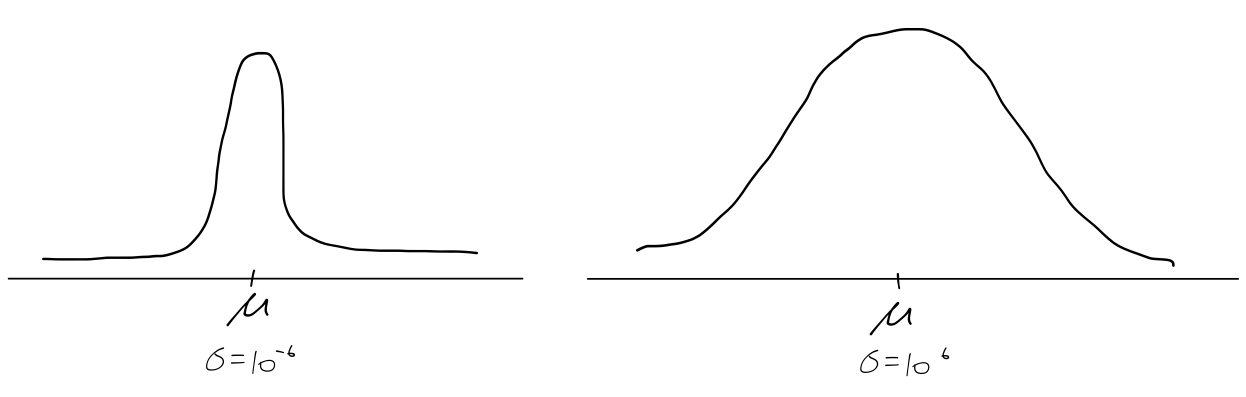
\includegraphics[height=5cm, width=13cm]{image_mle.png}

As the picture depicts above, the distribution with lower variance is more concentrated, implying having abundant information, while the other with higher variance is more like dispersed, meaning there is little information contains.\\

Before closing the section, let me introduce four interesting points about Fisher information.
\begin{itemize}
  \item Since Fisher information is a fundamental property of $pdf_\theta$, every $pdf_\theta$ has to have a Fisher information regardless of the type of distribution. 
  \item In case of normal distribution, in practice, people don't know what $\sigma^2$ is, when it comes to computation of Fisher information, so MLE estimation of $\sigma^2$ is used to plug.
  \item In general, people compute Fisher information just to see its form in order to check variability of the sample.
  \item Fisher information can be computed with respect to each separate parameter, such as $\mu$ and $\sigma^2$ for normal distribution. 
\end{itemize}

\textbf{Example} \quad Compute Fisher information for $\sigma^2$ in $n$ $i.i.d.$ samples from normal distribution $N(\mu, \sigma^2)$\\

Let a = $\sigma^2$, and recall the formula for Fisher information
$$I(a) = -E\left[\frac{d^2}{d\theta^2}\;\log\;pdf_\theta (X_i)\right]$$
$$\log \; pdf(X_i) = \frac{-\log\;(2\pi\sigma^2)}{2} - \frac{(X_i-\mu)^2}{2\sigma^2} = \frac{-\log\;(2\pi a)}{2} - \frac{(X_i-\mu)^2}{2\sigma^2}$$
$$\frac{d}{da}: \; -\frac{1}{2a} + \frac{(X_i-\mu)^2}{2a^2} \qquad \frac{d^2}{da^2}: \; \frac{1}{2a^2} - \frac{(X_i-\mu)^2}{a^3}$$
Hence, 
$$I(a) = -E\left[\frac{1}{2a^2} - \frac{(X_i-\mu)^2}{a^3}\right] = -\frac{1}{2a^2} + \frac{1}{a^3}E[(X_i - \mu)^2] = -\frac{1}{2a^2} + \frac{1}{a^3}{\sigma^2} = \frac{1}{2\sigma^4}$$

\subsubsection{Asymptotic Variance}
Asymptotic variance is used for measuring the variability and precision of estimated parameter(s). In asymptotic sense, as $n$ goes to $\infty$, asymptotic variance is defined as below.
$$Var(\hat{\theta}_{MLE}) \approx \frac{1}{nI(\theta)}$$

\textbf{Example} \quad $n$ $i.i.d.$ normal N($\mu,\sigma^2)$ samples\\

As for MLE estimator of $\mu$
$$\hat{\mu}_{MLE} = \frac{1}{n}\sum_{i=1}^n X_i = \bar{X} \qquad I(\hat{\mu}_{MLE}) = \frac{1}{\sigma^2}$$
Given the formula of asymptotic variance above, we obtain
$$Var(\hat{\mu}_{MLE}) \approx \frac{1}{n(\frac{1}{\sigma^2})} = \frac{\sigma^2}{n}$$ 
The asymptotic variance we obtained implies the precision and variability of the parameter $\hat{\mu}_{MLE}$. Then, we plug in MLE estimation of $\mu$ into the obtained asymptotic variance to estimate its precision/variability as follows.
$$\widehat{Var}(\hat{\mu}_{MLE}) = \frac{\hat{\sigma^2}}{n}$$
Repeating the process used to obtain asymptotic variance for MLE estimator of $\mu^2$, the asymptotic variance for $\sigma^2$ also will be hold as follows.
$$\hat{\sigma}_{MLE} = \frac{1}{n} \sum_{i=1}^n (X_i-\hat{\mu}_{MLE})^2 \qquad
I(\hat{\sigma}_{MLE}) = \frac{1}{2\sigma^4}$$
$$Var(\hat{\sigma^2}_{MLE}) \approx \frac{1}{n(\frac{1}{2\sigma^4})} = \frac{2\sigma^4}{n} \qquad \widehat{Var}(\hat{\sigma}^2_{MLE}) = \frac{2\hat{\sigma}^4_{MLE}}{n}$$

\textbf{Example} \quad $X_1, ... , X_n \stackrel{iid}{\sim} Pois(\lambda)$
As for MLE estimator of $\lambda$
$$\hat{\lambda}_{MLE} = \frac{1}{n}\sum_{i=1}^n X_i = \bar{X} \qquad I(\lambda) = -E\left[\frac{d^2}{d\lambda^2}\;\log\;pdf_\lambda (X_i)\right]$$
Recall $pdf$ of Poisson distribution
$$pdf_\lambda(X_i) = \frac{\lambda^{X_i}e^{-\lambda}}{X_i!}$$
$$\log \; pdf_\lambda (X_i) = X_i\;\log(\lambda) -\lambda - \log(X_i!)$$

$$\frac{d}{d\lambda}: \frac{X_i}{\lambda} - 1 \qquad \frac{d^2}{d\lambda^2}: \frac{-X_i}{\lambda^2} \Rightarrow I(\lambda) = -E\left[\frac{-X_i}{\lambda^2}\right] = \frac{1}{\lambda^2}E(X_i) = \frac{1}{\lambda}$$

$$Var(\hat{\lambda}_{MLE}) \approx \frac{1}{nI(\lambda)} = \frac{1}{n\cdot\frac{1}{\lambda}} = \frac{\lambda}{n} \qquad \widehat{Var}(\hat{\lambda}_{MLE}) = \frac{\hat{\lambda}_{MLE}}{n}$$

\textbf{Example} \quad $n$ $i.i.d.$ from $pdf_\alpha (X_i) = \frac{\Gamma(2\alpha)}{\Gamma(\alpha)^2}[X_i(1-X_i)]^{\alpha -1}$
$$\log\;pdf(X_i) = \log\;[\Gamma(2\alpha)] - 2\log[\Gamma(\alpha)] + (\alpha - 1)\log[X_i(1-X_i)]$$

$$\frac{d}{d\alpha}:\; \frac{1}{\Gamma(2\alpha)} \cdot \frac{d}{d\alpha}\Gamma(2\alpha) - \left[\frac{2}{\Gamma(\alpha)}\frac{d}{d\alpha}\Gamma(\alpha)\right]+\log(X_i(1-X_i)) =$$
$$2\frac{d}{d\alpha}\Gamma(\alpha)\left[\frac{1}{\Gamma(2\alpha)}-\frac{1}{\Gamma\alpha}\right]+\log(X_i(1-X_i))$$

$$\frac{d^2}{d\alpha^2}:\; 2\frac{d^2}{d\alpha^2}\Gamma\alpha[\frac{1}{\Gamma(2\alpha)}-\frac{1}{\Gamma(\alpha)}]+2\frac{d}{d\alpha}\Gamma(\alpha)\left[\frac{-2}{\Gamma(2\alpha)}\frac{d}{d\alpha}\Gamma(\alpha)+\frac{1}{\Gamma\alpha}\frac{d}{d\alpha}(\Gamma\alpha)\right]=$$
$$2\frac{d^2}{d\alpha^2}\Gamma\alpha\left[\frac{1}{\Gamma(2\alpha)}\right] + 2\left(\frac{d}{d\alpha}\Gamma\alpha\right)^2\left[\frac{1}{\Gamma\alpha^2}-\frac{2}{\Gamma(2\alpha)^2}\right] = -I(\alpha)$$
Note that since $X_i$ of $pdf$ does not exists in the second derivative of $\log\,pdf(X_i)$, its second derivative itself is equal to $-I(\theta)$ regardless of expectation.\\
$$Var(\hat{\alpha}_{MLE}) \approx \frac{1}{nI(\alpha)} \qquad \widehat{Var}(\hat{\alpha}_{MLE}) = \frac{1}{nI(\hat{\alpha}_{MLE})}$$

\subsubsection{Asymptotic Normality}
For most $\hat{\theta}_{MLE}$, $\hat{\theta}_{MLE} \sim N(\theta, \frac{1}{nI(\theta)})$ implies that its distribution is centered around true mean $\mu$ with variability of $Var(\hat{\theta}_{MLE})$. Otherwise, this can be expressed more formally as below.
$$\sqrt{nI(\theta)}\;(\hat{\theta}_{MLE}-\theta)  \xrightarrow{as\; n \rightarrow \infty} N(0,1)$$

\textbf{Implication}
\begin{itemize}
	\item As $n$ is close to $\infty$, MLE estimator $\hat{\theta}_{MLE}$ approaches to the true parameter $\theta$. This property shows that MLE estimation is a good method for parameter estimation.
    \item As long as we obtained MLE estimators and Fisher information, the confidence interval can be found using the one single formula as below.
    $$\hat{\theta}_{MLE} \pm z_{1-\frac{\alpha}{2}}\sqrt{\frac{1}{nI(\hat{\theta}_{MLE})}}$$
    For example, suppose that there is an $i.i.d.$ and normally distributed set of data $X_1,...,X_n$ with mean $\mu$ and variance $\sigma^2$. Recall that MLE estimator of $\mu$ in normal distribution is $\bar{X}$ and its Fisher information is $\frac{1}{\sigma^2}$. Hence, its 95\% confidence interval is defined as below.
$$\hat{\mu}_{MLE} \pm 1.96\sqrt{\frac{1}{n\cdot\frac{1}{\hat{\sigma^2}_{MLE}}}} \Leftrightarrow \hat{\mu}_{MLE} \pm 1.96\sqrt{\frac{\hat{\sigma}^2_{MLE}}{n}}$$
\end{itemize}








\end{section}
\end{document}


